\section{Team Members and Workloads}

The project is developed by \textbf{Group LHPD2}, consisting of the following members:

\begin{center}
    \renewcommand{\arraystretch}{1.5}
    \begin{tabularx}{\textwidth}{||c|c|c|X||}
    \hline
    \textbf{No.} & \textbf{Full Name} & \textbf{Student ID} & \textbf{Task Assigned} \\
    \hline
    1 & Nguyen Quang Phu & 2252621 & Team leader; Repository management; Ensure project timeline and verify work. \\
    \hline
    2 & Pham Huynh Bao Dai & 2252139 & Data preparation; Data preprocessing; Feature engineering; Document Data Processing. \\
    \hline
    3 & Nguyen Thanh Dat & 2252145 & Model implementation (Decision Tree, Random Forest); Training and evaluation; Document Model Implementation. \\
    \hline
    4 & Nguyen Tien Hung & 2252280 & Model implementation (SVM, Logistic Regression); Training and evaluation; Document Model Implementation. \\
    \hline
    5 & Nguyen Thien Loc & 2252460 & Model evaluation, hyperparameter tuning, Model comparison, Document Performance Analysis. \\
    \hline
    \end{tabularx}
\end{center} 

\section{Project Organization and Requirements}

The project follows structured collaboration and software engineering practices, adhering to the following guidelines:

\subsection{Team Collaboration and Version Control}

\begin{itemize}
    \item Each member actively contributes to the repository, ensuring distributed workload and participation.
    \item The main repository is hosted on GitHub at:  
    \textbf{\url{https://github.com/pdz1804/ML_LHPD2}}.
    \item The repository follows a branching strategy, where each member develops on a dedicated branch and submits changes via pull requests.
    \item Code reviews and discussions are conducted to ensure quality, maintainability, and adherence to best practices.
    \item Version control best practices are maintained, with regular commits, documentation, and codebase integrity.
\end{itemize}

\subsection{GitHub Repository Structure}

The repository is structured to support multiple problem formulations, model implementations, and comparative analyses while maintaining a clean code structure and proper documentation.

\begin{itemize}
    \item \textbf{Main repository}: Created and maintained by a designated team member.
    \item \textbf{Forking workflow}: Other members fork and contribute via pull requests.
    \item \textbf{Branching strategy}: Different branches are created for models and features to ensure isolated development.
    \item \textbf{Comprehensive documentation}: Ensures clarity in problem definitions, methodologies, and results.
\end{itemize}

\subsection{Key Requirements}

\begin{itemize}
    \item \textbf{Clear problem documentation}: Problem statements and their variations are well-documented.
    \item \textbf{Consistent implementation interface}: All models follow a standardized interface to ensure ease of comparison.
    \item \textbf{Comprehensive testing}: Each component undergoes rigorous testing.
    \item \textbf{Detailed comparative analysis}: Models are evaluated across multiple performance metrics.
    \item \textbf{Regular code reviews and pull requests}: Maintains code integrity and quality.
    \item \textbf{Version control best practices}: Ensures organized and maintainable development.
\end{itemize}

\section{Repository Structure}

To facilitate maintainability, scalability, and efficient collaboration, the repository follows a structured layout:

\begin{figure}[H]
    \centering
    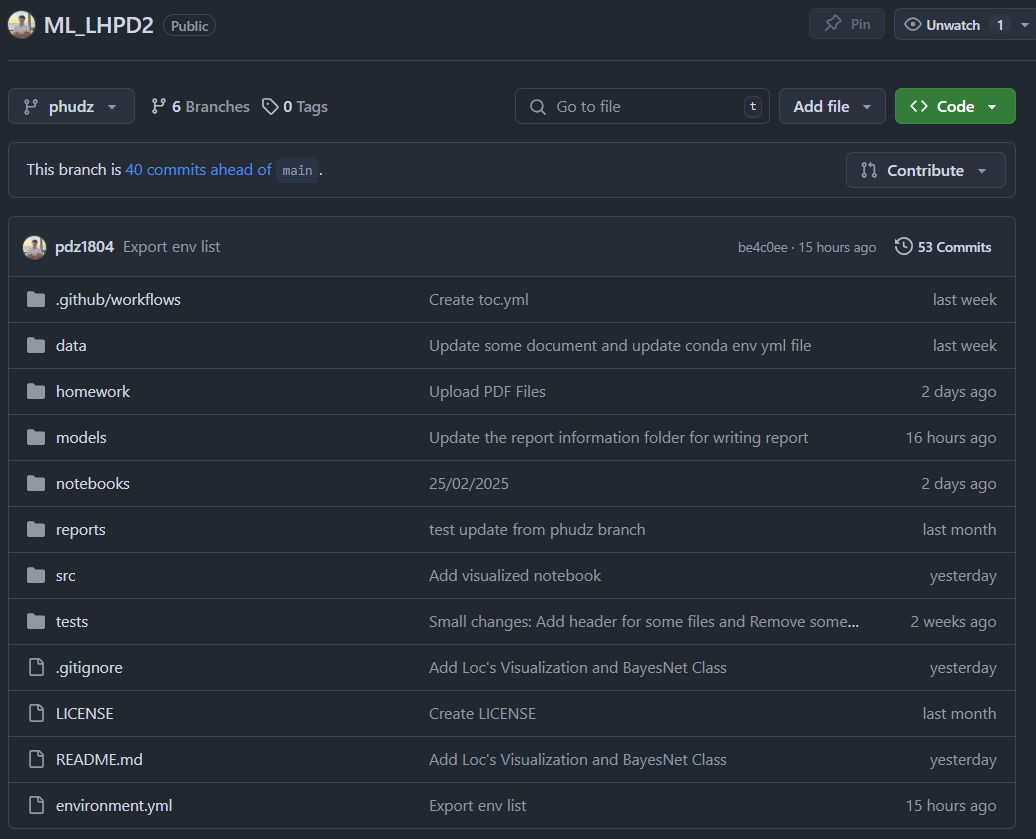
\includegraphics[width=\textwidth]{img/progress/github_repo.PNG}
    \caption{Github Repository Structure}
    \label{fig:github-repo}
\end{figure}

\newpage
